\documentclass[../main.tex]{subfiles}

\begin{document}

% ====================================================
% p.1 表紙
% ====================================================
\begin{center}
  {\Large 東大理科数学 1977}
\end{center}

\newpage

% ====================================================
% p.2 第1問
% ====================================================
\subsection*{第1問}

[解] $g(x) = x^3 - 3kx$ とおくと $g'(x) = 3x^2 - 3k$ から, $k$ によって下表を考える。

\begin{enumerate}
  \item[$1^\circ$] $k > 0$
    \[
      \begin{array}{c|c|c|c|c|c}
        x & \dots & -\sqrt{k} & \dots & \sqrt{k} & \dots \\ \hline
        g' & + & 0 & - & 0 & + \\ \hline
        g & \nearrow & \text{極大} & \searrow & \text{極小} & \nearrow
      \end{array}
    \]
  \item[$2^\circ$] $k \le 0$

    $g(x)$ は単調増加
\end{enumerate}

$f(x)$ は偶関数だから, $0 \le x \le 1$ でしらべればよい。

$1^\circ$ の時
\begin{enumerate}
  \item[(i)] $0 < \sqrt{k} \le 1 \iff 0 < k \le 1$ の時

    $f(x)$ の最大値のコウホは, $f(0), f(\sqrt{k}), f(1)$ である。
    \[
      f(1) = |1-3k|, \quad f(0) = 0, \quad f(\sqrt{k}) = 2k^{\frac{3}{2}}
    \]

  \item[(ii)] $1 \le \sqrt{k} \iff 1 \le k$ の時

    $f(x)$ の最大値のコウホは, $f(0) = 0, f(1) = |1-3k|$
\end{enumerate}

$2^\circ$ の時

$f(x)$ のコウホは $f(0) = 0, f(1) = |1-3k|$

以上まとめて, $y = M(k)$ のグラフは以下

\begin{center}
  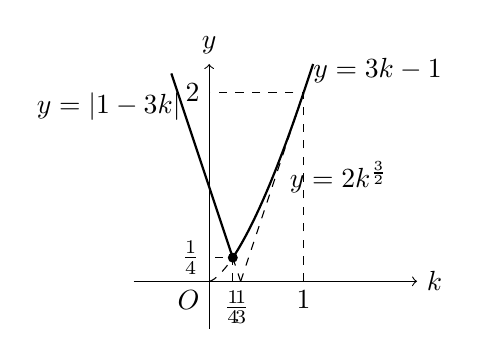
\begin{tikzpicture}[scale=1.2]
    % Axes
    \draw[->] (-0.8,0) -- (2.2,0) node[right] {$k$};
    \draw[->] (0,-0.5) -- (0,2.3) node[above] {$y$};
    \node[below left] at (0,0) {$O$};

    % Solid curve for M(k)
    % k <= 1/4: y = 1 - 3k
    \draw[thick,domain=-0.4:0.25] plot (\x, {1 - 3*\x});
    % 1/4 <= k <= 1: y = 2 k^(3/2)
    \draw[thick,domain=0.25:1,samples=50] plot (\x, {2*\x^(1.5)});
    % k >= 1: y = 3k - 1
    \draw[thick,domain=1:1.1,samples=10] plot (\x, {3*\x - 1});

    % Labels for functions
    \node[above left] at (-0.2,1.6) {$y=|1-3k|$};
    \node[right] at (0.75,1.1) {$y=2k^{\frac{3}{2}}$};
    \node[above right] at (1.0,2.0) {$y=3k-1$};

    % Dashed extending lines
    \draw[dashed,domain=0.25:0.3333] plot (\x, {1 - 3*\x});
    \draw[dashed,domain=0.3333:1] plot (\x, {3*\x - 1});
    \draw[dashed,domain=0:0.25,samples=30] plot (\x, {2*\x^(1.5)});

    % Key values on axes
    \draw[dashed] (0.25,0) node[below] {$\frac{1}{4}$} -- (0.25,0.25) -- (0,0.25) node[left] {$\frac{1}{4}$};
    \draw[dashed] (0.3333,0) node[below] {$\frac{1}{3}$} -- (0.3333,0);
    \draw[dashed] (1,0) node[below] {$1$} -- (1,2) -- (0,2) node[left] {$2$};

    \fill (0.25,0.25) circle (1.5pt);
  \end{tikzpicture}
\end{center}

よって, $\min M(k) = M\left(\frac{1}{4}\right) = \frac{1}{4}$

\newpage

% ====================================================
% p.3 第2問
% ====================================================
\subsection*{第2問}

[解] $a_1, a_2, b_1, b_2 \in \mathbb{Q} \quad \dots *$

\begin{itemize}
  \item $a = \sqrt{a_1^2 + a_2^2}, \quad b = \sqrt{b_1^2 + b_2^2}, \quad c = \overline{AB} = \sqrt{(a_1 - b_1)^2 + (a_2 - b_2)^2}$
  \item $\cos\theta = \frac{a^2 + b^2 - c^2}{2ab}, \quad \sin\theta = \frac{|a_1 b_2 - a_2 b_1|}{ab} \quad \dots \text{①}$
\end{itemize}

である。$a^2, b^2, c^2 \in \mathbb{Q}$ に

\begin{enumerate}
  \item[(i)] $ab \in \mathbb{Q}$ の時、$a^2, b^2, c^2 \in \mathbb{Q}$ と ①から
    \[
      \text{(i)} \to \text{(ii)}, \quad \text{(i)} \to \text{(iii)}
    \]
    が成り立つ。

  \item[(ii)] $\cos\theta \in \mathbb{Q}$ の時
    \begin{enumerate}
      \item[(A)] $\cos\theta \neq 0$ なら、①から $ab \in \mathbb{Q}$ である ($\because *$ )
      \item[(B)] $\cos\theta = 0$ なら、$\sin\theta = \pm 1$ であり、①から $ab \in \mathbb{Q}$ である ($\because *$ )
    \end{enumerate}
    以上から $\text{(ii)} \to \text{(i)}$ が成り立つ。

  \item[(iii)] $\sin\theta \in \mathbb{Q}$ の時
    \begin{enumerate}
      \item[(A)] $\sin\theta \neq 0$ なら、同様に $ab \in \mathbb{Q}$
      \item[(B)] $\sin\theta = 0$ なら、$\cos\theta = \pm 1$ となり、同様に $ab \in \mathbb{Q}$
    \end{enumerate}
    以上から、$\text{(iii)} \to \text{(i)}$ が成り立つ。
\end{enumerate}

したがって、$\text{(i)} \iff \text{(ii)}$, $\text{(i)} \iff \text{(iii)}$ だから、$\text{(ii)} \iff \text{(iii)}$ であり、示された。

\newpage

% ====================================================
% p.4 第3問（検討メモ）
% ====================================================
\subsection*{第3問（検討メモ）}

% [構想メモ]
% r(P)は X, Y の2変数関数。
% → 円が A, B, C に含まれる条件
% r <= X, r <= Y, r <= 1/2(-\sqrt{3}X + \sqrt{3} - Y)
% の値域を1変数消してグラフに表し, そのうち max をとっていけば良いが...
% 1つ注意すべきは

\newpage

% ====================================================
% p.5 第3問
% ====================================================
\subsection*{第3問}

[解] $P(X,Y)$ とおく。$l: y = -\sqrt{3}x + \sqrt{3}$ とおく。

\begin{center}
  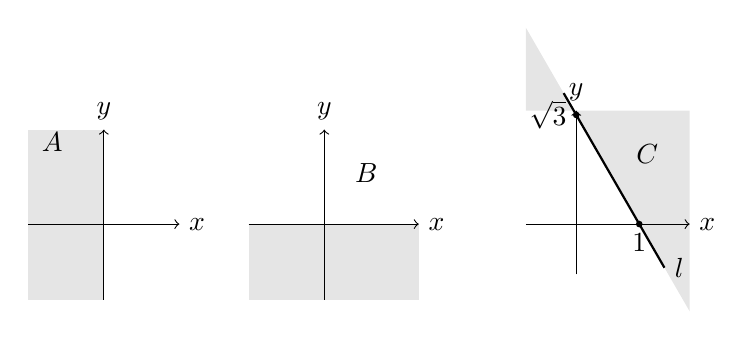
\begin{tikzpicture}[scale=0.8]
    % Region A
    \begin{scope}[shift={(0,0)}]
      \fill[gray!20] (-1.2,-1.2) rectangle (0,1.5);
      \draw[->] (-1.2,0) -- (1.2,0) node[right] {$x$};
      \draw[->] (0,-1.2) -- (0,1.5) node[above] {$y$};
      \node[above left] at (-0.5,1.0) {$A$};
    \end{scope}

    % Region B
    \begin{scope}[shift={(3.5,0)}]
      \fill[gray!20] (-1.2,-1.2) rectangle (1.5,0);
      \draw[->] (-1.2,0) -- (1.5,0) node[right] {$x$};
      \draw[->] (0,-1.2) -- (0,1.5) node[above] {$y$};
      \node[above left] at (1.0,0.5) {$B$};
    \end{scope}

    % Region C
    \begin{scope}[shift={(7.5,0)}]
      \fill[gray!20] (-0.8,{sqrt(3)*(1+0.8)}) -- (1.8,{sqrt(3)*(1-1.8)}) -- (1.8,1.8) -- (-0.8,1.8) -- cycle;
      \draw[->] (-0.8,0) -- (1.8,0) node[right] {$x$};
      \draw[->] (0,-0.8) -- (0,1.8) node[above] {$y$};
      \draw[thick] (-0.2,{sqrt(3)*(1+0.2)}) -- (1.4,{sqrt(3)*(1-1.4)}) node[right] {$l$};
      \node[above right] at (0.8,0.8) {$C$};
      \node[left] at (0,{sqrt(3)}) {$\sqrt{3}$};
      \node[below] at (1,0) {$1$};
      \fill (0,{sqrt(3)}) circle (1.5pt);
      \fill (1,0) circle (1.5pt);
    \end{scope}
  \end{tikzpicture}
\end{center}

(1) $P$ が下図斜線部をうごく時、$Y < 0 \quad (0 \le X \le 1)$ または $Y \le -\sqrt{3}X + \sqrt{3} \quad (1 < X)$ とかける。

\begin{enumerate}
  \item[$1^\circ$] 円が $A$ に含まれる時
    \[
      r \le X
    \]
  \item[$2^\circ$] 円が $C$ に含まれる時
    \[
      r \le \frac{|\sqrt{3}X + Y - \sqrt{3}|}{\sqrt{1+3}} = \frac{1}{2}(-\sqrt{3}X - Y + \sqrt{3})
    \]
\end{enumerate}

だから、$\alpha, \beta$ のうち小さくない方を $\max\{\alpha, \beta\}$ と表すと、
\[
  r(P) = \max\left\{ X, \frac{1}{2}(-\sqrt{3}X - Y + \sqrt{3}) \right\}
\]
である。$X$ を固定して、$Y$ をうごかすと $-\sqrt{3}X - Y + \sqrt{3}$ は $Y$ の単調減少関数だから、
\[
  -\sqrt{3}X - Y + \sqrt{3}
  \begin{cases} > -\sqrt{3}X + \sqrt{3} & (0 \le X \le 1) \\ \ge 0 & (1 < X)
  \end{cases}
\]
だから、$r(P)$ のグラフは右図のようになり、
\[
  r(P) \ge -3 + 2\sqrt{3}
\]

(2) $P$ の場所を以下のように場合分けする。この時、$A \cup B \cup C$ は平面全体を表すことに注意する。又、以下境界は全て含むとする。

\begin{center}
  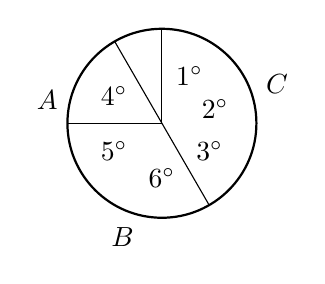
\begin{tikzpicture}[scale=1.0]
    \draw[thick] (0,0) circle (1.2cm);
    \draw (0,0) -- (0,1.2);
    \draw (0,0) -- (-1.2,0);
    \draw (0,0) -- (120:1.2cm);
    \draw (0,0) -- (-60:1.2cm);
    \node at (60:0.7cm) {$1^\circ$};
    \node at (15:0.7cm) {$2^\circ$};
    \node at (150:0.7cm) {$4^\circ$};
    \node at (210:0.7cm) {$5^\circ$};
    \node at (270:0.7cm) {$6^\circ$};
    \node at (330:0.7cm) {$3^\circ$};
    \node[left] at (-1.2,0.3) {$A$};
    \node[below] at (-0.5,-1.2) {$B$};
    \node[right] at (1.2,0.5) {$C$};
  \end{tikzpicture}
\end{center}

\begin{enumerate}
  \item[$1^\circ$] $P$ が $A \cap B \cap C$ をうごく時
    \[
      0 \le Y \le -\sqrt{3}X + \sqrt{3} \quad (0 \le X \le 1)
    \]
    である。
    \begin{align*}
      A \text{ に含まれる} &\dots r \le X \\
      B \text{ に含まれる} &\dots r \le Y \\
      C \text{ に含まれる} &\dots r \le \frac{1}{2}(-\sqrt{3}X - Y + \sqrt{3})
    \end{align*}
    だから、$r(P) = \max\left\{ X, Y, \frac{1}{2}(-\sqrt{3}X - Y + \sqrt{3}) \right\}$ である。まず、
    \[
      Y \ge \frac{1}{2}(-\sqrt{3}X - Y + \sqrt{3}) \iff Y \ge \frac{1}{3}(-\sqrt{3}X + \sqrt{3})
    \]
    だから、
    \[
      \begin{cases}
        0 \le Y \le \frac{1}{3}(-\sqrt{3}X + \sqrt{3}) \text{ の時 } r(P) = \max\left\{ X, \frac{1}{2}(-\sqrt{3}X - Y + \sqrt{3}) \right\} & \dots \text{1-①} \\
        \frac{1}{3}(-\sqrt{3}X + \sqrt{3}) \le Y \le \sqrt{3}(-X + 1) \text{ の時 } r(P) = \max \{ X, Y \} & \dots \text{1-②}
      \end{cases}
    \]
    で $X$ を固定して $Y$ をうごかすと、
    \begin{align*}
      \text{1-①の時} \quad &\frac{1}{3}\sqrt{3}(-X+1) \le \frac{1}{2}(-\sqrt{3}X - Y + \sqrt{3}) \le \frac{\sqrt{3}}{2}(-X+1) \\
      \text{1-②の時} \quad &\frac{1}{3}\sqrt{3}(-X+1) \le Y \le \sqrt{3}(-X+1)
    \end{align*}
    でグラフは右図で
    \[
      r(P) \ge \frac{-1 + \sqrt{3}}{2} \quad \dots *
    \]

  \item[$2^\circ$] $P$ が $A \cap B \cap \overline{C}$ をうごく時

    $A$ に含まれる $\dots r \le X$, $B$ に含まれる $\dots r \le Y$ から、
    $r(P) = \max(X, Y)$ であり、又
    \[
      \begin{cases}
        \frac{1}{\sqrt{3}}(-\sqrt{3}X + \sqrt{3}) \le Y & (0 \le X \le 1) \\
        0 \le Y & (1 \le X)
      \end{cases}
    \]
    だから、グラフは右図で
    \[
      r(P) \ge \frac{1}{2}(3 - \sqrt{3}) \quad \dots *
    \]

  \item[$3^\circ$] $P$ が $\overline{A} \cap B \cap C$ をうごく時

    $B$ に含まれる $\dots r \le Y$, $C$ に含まれる $\dots r \le \frac{1}{2}(-\sqrt{3}X - Y + \sqrt{3})$ で、$0 \le Y \le \sqrt{3}(-X+1) \quad (X \le 0)$ である。よって、
    \[
      \begin{cases}
        0 \le Y \le \frac{\sqrt{3}}{3}(-X+1) \text{ の時 } r(P) = \frac{1}{2}(-\sqrt{3}X - Y + \sqrt{3}) \\
        \frac{\sqrt{3}}{3}(-X+1) \le Y \le \sqrt{3}(-X+1) \text{ の時 } r(P) = Y
      \end{cases}
    \]
    左図から、
    \[
      r(P) \ge \frac{\sqrt{3}}{3} \quad \dots *
    \]

  \item[$4^\circ$] $P$ が $A \cap \overline{B} \cap \overline{C}$ をうごく時

    $1 \le X$ で、$r(P) = X$ から
    \[
      r(P) \ge 1 \quad \dots *
    \]

  \item[$5^\circ$] $P$ が $\overline{A} \cap \overline{B} \cap \overline{C}$ をうごく時

    $1 \le Y$ で、$r(P) = Y$ から
    \[
      r(P) \ge 1 \quad \dots *
    \]

  \item[$6^\circ$] $P$ が $\overline{A} \cap \overline{B} \cap C$ をうごく時

    $X, Y \le 0$ で、$r(P) = \frac{1}{2}(-\sqrt{3}X - Y + \sqrt{3})$ から
    \[
      r(P) \ge \frac{\sqrt{3}}{2} \quad \dots *
    \]
\end{enumerate}

以上 $1^\circ \sim 6^\circ$ から、
\[
  \min r(P) = \frac{-1 + \sqrt{3}}{2}
\]

\newpage

% ====================================================
% p.6 第4問
% ====================================================
\subsection*{第4問}

[解]
\begin{center}
  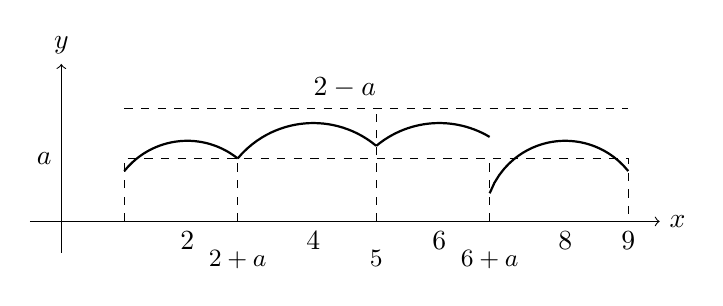
\begin{tikzpicture}[scale=0.8]
    \draw[->] (-0.5,0) -- (9.5,0) node[right] {$x$};
    \draw[->] (0,-0.5) -- (0,2.5) node[above] {$y$};

    \node[below] at (2,0) {$2$};
    \node[below] at (4,0) {$4$};
    \node[below] at (6,0) {$6$};
    \node[below] at (8,0) {$8$};
    \node[below] at (9,0) {$9$};
    \node[below] at (2.8, -0.3) {\small $2+a$};
    \node[below] at (5, -0.3) {\small $5$};
    \node[below] at (6.8, -0.3) {\small $6+a$};

    \node[left] at (0, 1.0) {$a$};
    \node[above] at (4.5, 1.8) {$2-a$};

    \draw[dashed] (1,0) -- (1,1.0) -- (9,1.0) -- (9,0);
    \draw[dashed] (1,1.8) -- (9,1.8);
    \draw[dashed] (2.8,0) -- (2.8,1.0);
    \draw[dashed] (5,0) -- (5,1.8);
    \draw[dashed] (6.8,0) -- (6.8,1.0);

    % arcs
    \draw[thick, domain=1:2.8, samples=30] plot (\x, {sqrt(max(0, 1.64 - (\x-2)^2))});
    \draw[thick, domain=2.8:5, samples=30] plot (\x, {sqrt(max(0, 2.44 - (\x-4)^2))});
    \draw[thick, domain=5:6.8, samples=30] plot (\x, {sqrt(max(0, 2.44 - (\x-6)^2))});
    \draw[thick, domain=6.8:9, samples=30] plot (\x, {sqrt(max(0, 1.64 - (\x-8)^2))});
  \end{tikzpicture}
\end{center}

$C$ の方程式は
\[
  C:
  \begin{cases}
    (x-2)^2 + y^2 = 1+a^2 & (1 \le x \le 2+a) \\
    (x-4)^2 + y^2 = (2-a)^2 + 1 & (2+a \le x \le 5) \\
    (x-6)^2 + y^2 = (2-a)^2 + 1 & (5 \le x \le 6+a) \\
    (x-8)^2 + y^2 = 1+a^2 & (6+a \le x \le 9)
  \end{cases}
\]
であり, $x=5$ を軸に対称だから, もとめる立体の $x \le 5$ の部分の体積 $\overline{V}(a)$ として,
\[
  V(a) = 2\overline{V}(a) \quad \dots \text{①}
\]
であり
\begin{align*}
  \overline{V}(a) &= \int_{-1}^a \pi \left[ (1+a^2) - x^2 \right] dx + \int_{a-2}^1 \pi \left\{ (a^2-4a+5) - x^2 \right\} dx \\
  &= \pi \left[ (1+a^2)x - \frac{1}{3}x^3 \right]_{-1}^a + \pi \left[ (a^2-4a+5)x - \frac{1}{3}x^3 \right]_{a-2}^1 \\
  &= \pi \left[ (1+a^2)\cdot a - \frac{1}{3}a^3 + (1+a^2) - \frac{1}{3} \right] \\
  &\quad + \pi \left[ (a^2-4a+5) - \frac{1}{3} - (a^2-4a+5)(a-2) + \frac{1}{3}(a-2)^3 \right] \\
  &= \pi \left[ \frac{2}{3}a^3 + a^2 + a + \frac{2}{3} + a^2 - 4a + 5 - \frac{1}{3} - (a-2)\left\{ a^2-4a+5 - \frac{1}{3}(a-2)^2 \right\} \right] \\
  &= \pi \left[ \frac{2}{3}a^3 + 2a^2 - 3a + 5 + \frac{1}{3} - (a-2)\left( \frac{2}{3}a^2 - \frac{8}{3}a + \frac{11}{3} \right) \right] \\
  &= \pi \left[ \frac{2}{3}a^3 + 2a^2 - 3a + 5 + \frac{1}{3} - \frac{2}{3}a^3 + \frac{8}{3}a^2 - \frac{11}{3}a + \frac{4}{3}a^2 - \frac{16}{3}a + \frac{22}{3} \right] \\
  &= \pi \left[ 6a^2 - 12a + \frac{38}{3} \right] \\
  &= \pi \left[ 6(a-1)^2 + \frac{20}{3} \right]
\end{align*}
より, $0 \le a \le 2$ のとき
\[
  \min V(a) = 2\overline{V}(1) = \frac{40}{3}\pi
\]

% [本試のミス]
% ・最後の代入忘れ　書いてあったのにこれはひどい

\newpage

% ====================================================
% p.7 （白紙枠）
% ====================================================
\subsection*{}

% （白紙）

\newpage

% ====================================================
% p.8 第5問（新課程）
% ====================================================
\subsection*{第5-新問}

[解注] 行列 $A =
\begin{pmatrix} c & -s \\ s & c
\end{pmatrix}$ は $\theta$ 回転を表す行列である。

[解] $A(I-tJ) = I+tJ \dots \text{①}$ の左辺は, $I$ が単位行列であるから,
\[
  A(I-tJ) = AI - tAJ = A - tAJ = A - t
  \begin{pmatrix} -c & -d \\ a & b
  \end{pmatrix} \quad \dots \text{②}
\]
又, ①の右辺は
\[
  I + tJ =
  \begin{pmatrix} 1 & 0 \\ 0 & 1
  \end{pmatrix} + t
  \begin{pmatrix} 0 & -1 \\ 1 & 0
  \end{pmatrix} \quad \dots \text{③}
\]
である。①, ②, ③から, 行列の各成分を比較して,
\begin{align}
  a + ct &= 1 \label{eq:hw-5-4} \\
  b + dt &= -t \label{eq:hw-5-5} \\
  c - at &= t \label{eq:hw-5-6} \\
  d - bt &= 1 \label{eq:hw-5-7}
\end{align}
まず, \eqref{eq:hw-5-4} $\times t$ と \eqref{eq:hw-5-6} を辺々足して
\[
  c(t^2+1) = 2t \quad \therefore c = \frac{2t}{t^2+1}
\]
\eqref{eq:hw-5-4} に代入して,
\[
  a = 1 - ct = \frac{1-t^2}{1+t^2}
\]
次に \eqref{eq:hw-5-5} $\times t$ と \eqref{eq:hw-5-7} を辺々足して,
\[
  (1+t^2)d = 1 - t^2 \quad \therefore d = \frac{1-t^2}{1+t^2}
\]
\eqref{eq:hw-5-5} に代入して,
\[
  b = -(1+d)t = -\frac{2t}{t^2+1}
\]
以上から
\[
  (a,b,c,d) = \left( \frac{1-t^2}{1+t^2}, \, -\frac{2t}{t^2+1}, \, \frac{2t}{1+t^2}, \, \frac{1-t^2}{1+t^2} \right)
\]
が必要。これを \eqref{eq:hw-5-4} $\sim$ \eqref{eq:hw-5-7} に代入すると, いずれも成立し, 十分。よってこれが答えである。

さて, $-\pi < \theta < \pi$ に対し, $t = \tan\frac{\theta}{2}$ とおくと, $t$ は全実数をとり,
\[
  \begin{cases}
    \dfrac{1-t^2}{1+t^2} = \cos\theta \quad (= c \text{ とする}) \\[10pt]
    \dfrac{2t}{1+t^2} = \sin\theta \quad (= s \text{ とする})
  \end{cases}
\]
に注意すると,
\begin{align*}
  \begin{pmatrix} x \\ y
  \end{pmatrix} = A
  \begin{pmatrix} 3 \\ 4
  \end{pmatrix} &=
  \begin{pmatrix} c & -s \\ s & c
  \end{pmatrix}
  \begin{pmatrix} 3 \\ 4
  \end{pmatrix} =
  \begin{pmatrix} 3c-4s \\ 3s+4c
  \end{pmatrix} \\
  &= c
  \begin{pmatrix} 3 \\ 4
  \end{pmatrix} + s
  \begin{pmatrix} -4 \\ 3
  \end{pmatrix}
\end{align*}
となる。$
\begin{pmatrix} 3 \\ 4
\end{pmatrix} \perp
\begin{pmatrix} -4 \\ 3
\end{pmatrix}$ および $\left|
\begin{pmatrix} 3 \\ 4
\end{pmatrix} \right| = \left|
\begin{pmatrix} -4 \\ 3
\end{pmatrix} \right| = 5$, $-\pi < \theta < \pi$ から, 点 $(x,y)$ は, $(-3,-4)$ をのぞく, 原点中心半径5の円周上をうごく。

これを図示すると右図太線部
\begin{center}
  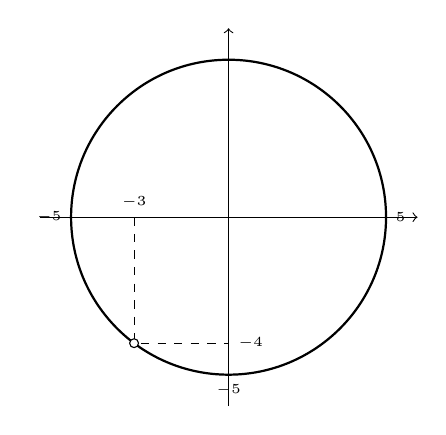
\begin{tikzpicture}[scale=0.4]
    \draw[->] (-6,0) -- (6,0);
    \draw[->] (0,-6) -- (0,6);
    \draw[thick] (0,0) circle (5);
    \draw[dashed] (-3,0) -- (-3,-4) -- (0,-4);
    \node[above] at (-3,0) {\tiny $-3$};
    \node[right] at (0,-4) {\tiny $-4$};
    \node[right] at (5,0) {\tiny $5$};
    \node[below] at (0,-5) {\tiny $-5$};
    \node[left] at (-5,0) {\tiny $-5$};
    \fill[white] (-3,-4) circle (4pt);
    \draw (-3,-4) circle (4pt);
  \end{tikzpicture}
\end{center}

\newpage

% ====================================================
% p.9 第5問（旧課程・白紙枠）
% ====================================================
\subsection*{第5問}

% （白紙）

\newpage

% ====================================================
% p.10 第6問（新課程）
% ====================================================
\subsection*{第6-新問}

[解] $l, m$ の方向ベクトル $\vec{l}, \vec{m}$ は各々
\[
  \vec{l} =
  \begin{pmatrix} 2 \\ 1 \\ 1
  \end{pmatrix} -
  \begin{pmatrix} 1 \\ 1 \\ 0
  \end{pmatrix} =
  \begin{pmatrix} 1 \\ 0 \\ 1
  \end{pmatrix}, \qquad
  \vec{m} =
  \begin{pmatrix} 1 \\ 3 \\ 2
  \end{pmatrix} -
  \begin{pmatrix} 1 \\ 1 \\ 1
  \end{pmatrix} =
  \begin{pmatrix} 0 \\ 2 \\ 1
  \end{pmatrix} \quad \dots \text{①}
\]
である。これらに垂直なベクトル $\vec{p}$ の1つに, $\vec{p} =
\begin{pmatrix} -2 \\ -1 \\ 2
\end{pmatrix}$ がある。$\quad \dots \text{②}$

\begin{enumerate}
  \item[(1)] ①, ②から,
    \[
      -2(x-1) + (-1)(y-1) + 2(z-0) = 0 \quad \therefore -2x-y+2z+3 = 0
    \]

  \item[(2)] $n$ 上の点を $X$ とする。$t$ をパラメータ, $a, b, c$ を定数として
    \[
      \overrightarrow{OX} =
      \begin{pmatrix} 2 \\ 0 \\ 1
      \end{pmatrix} + t
      \begin{pmatrix} a \\ b \\ c
      \end{pmatrix}
    \]
    とおける。これが $l, m$ と交わるので, $s, u \in \mathbb{R}$ として, ①から
    \[
      \begin{cases}
        \overrightarrow{OX} =
        \begin{pmatrix} 1 \\ 1 \\ 0
        \end{pmatrix} + s
        \begin{pmatrix} 1 \\ 0 \\ 1
        \end{pmatrix} \\
        \overrightarrow{OX} =
        \begin{pmatrix} 1 \\ 1 \\ 1
        \end{pmatrix} + u
        \begin{pmatrix} 0 \\ 2 \\ 1
        \end{pmatrix}
      \end{cases}
      \quad \dots \text{③}
    \]
    をみたす $s, u$ がある。対応する $t$ を各々 $t_1, t_2$ として,
    \[
      \begin{cases}
        2 + at_1 = 1 + s \\
        bt_1 = 1 \\
        1 + ct_1 = s
      \end{cases}
      \qquad
      \begin{cases}
        2 + at_2 = 1 \\
        bt_2 = 1 + 2u \\
        1 + ct_2 = 1 + u
      \end{cases}
    \]
    これをみたす $s, u, t_1, t_2$ の存在条件から, $a = b = c$ となり, この時 $s = 2, u = -1$ となるから ③に代入して
    \[
      \begin{cases}
        l \text{ と } n \dots (3,1,2) \\
        m \text{ と } n \dots (1,-1,0)
      \end{cases}
    \]
\end{enumerate}

\end{document}
